\title{Assignment 5.1}
\author{
        Pradyot Prakash - 130050008
            \\
        Utkarsh Mall - 130050037
			\\
		Samarth Mishra - 130260018
}
\date{\today}
\documentclass[11pt]{article}
\usepackage[left=2.5cm,top=2cm,right=2.5cm,bottom=2cm,bindingoffset=0.5cm]{geometry}
\usepackage{graphicx}
\usepackage{siunitx}
\usepackage{amsmath}
\usepackage[section]{placeins}
\graphicspath{ {../images/} }
\renewcommand\thesubsection{(\alph{subsection})}
\begin{document}
\maketitle

\subsection{}
Chosen value for $q = 3$

\subsection{}
Weight mask 
\FloatBarrier
\begin{figure}[h]
\centering
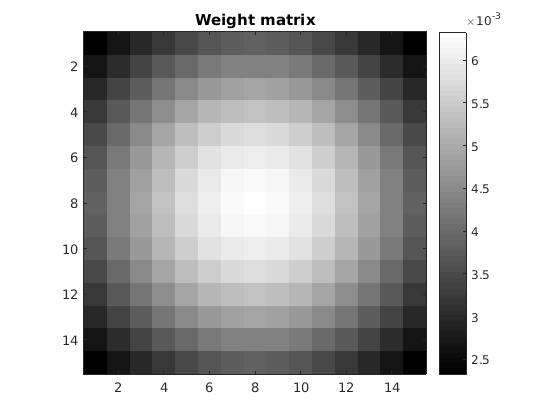
\includegraphics[scale=0.5]{weight}
\end{figure}

\subsection{}
Initial estimate of memberships are computed using the cluster means as calculated in the next part. Membership values are initilised using the standard FCM update, using the cluster means from kmeans and a constant bias. This makes sense because assuming the current cluster means, these are the membership values that optimise the objective function.
\begin{figure}[h]
\centering
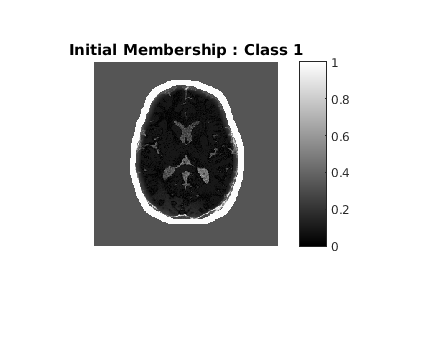
\includegraphics[]{init1}
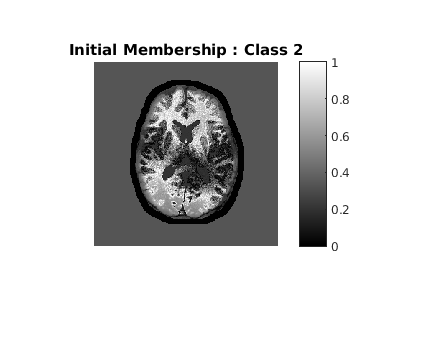
\includegraphics[]{init2}
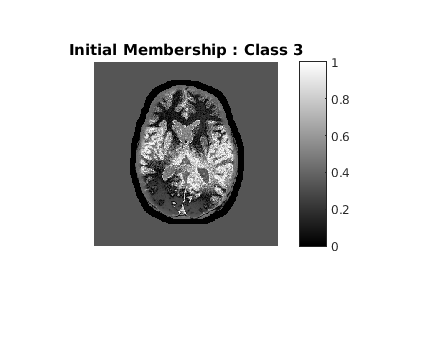
\includegraphics[]{init3}
\end{figure}

\FloatBarrier

\subsection{}
We initialised class means using the \textbf{kmeans} algorithm. Class means computed by FCM are expected to be close to the values computed by kmeans. \\
Initial cluster means for the three classes = [0.0027 ,   0.5775  ,  0.3757]

\subsection{}
Objective Funnction
\begin{figure}[h]
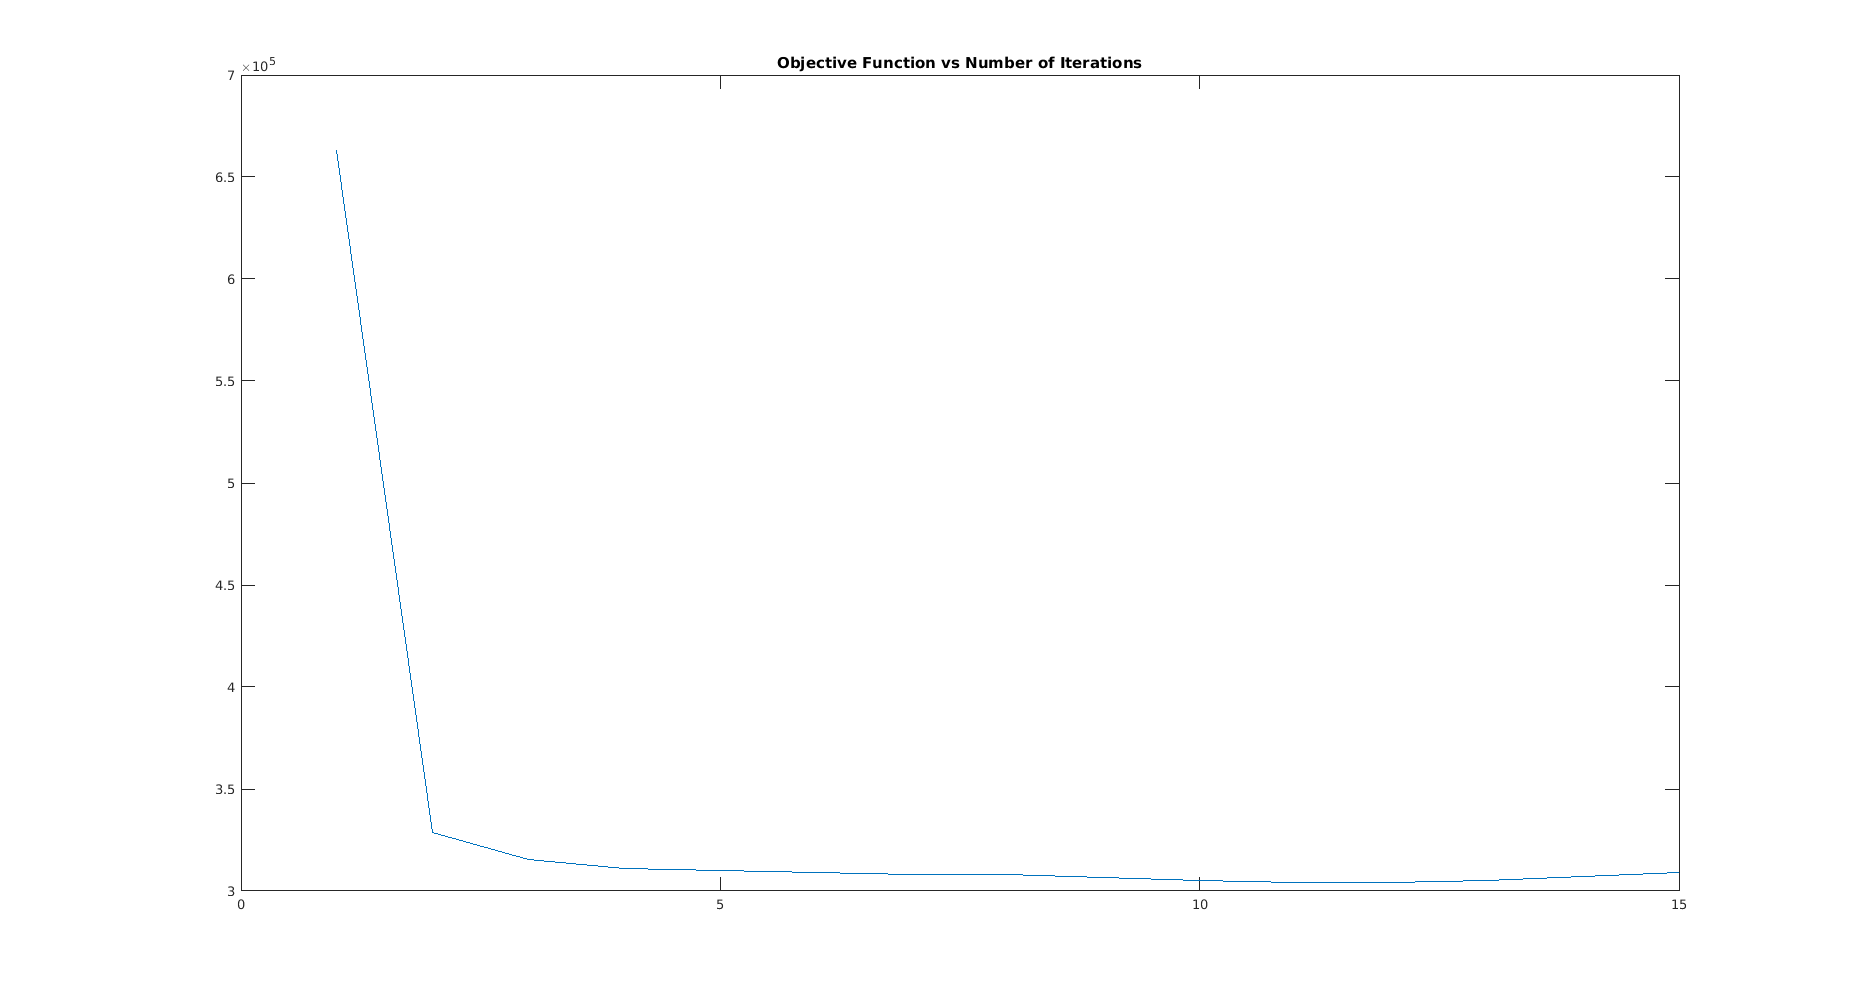
\includegraphics[scale=0.3]{objfun}
\end{figure}

\FloatBarrier

\subsection{}
After FCM optimisation

\begin{figure}[h]
\centering
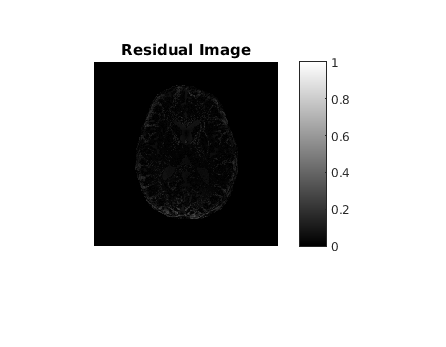
\includegraphics[]{residual}
\end{figure}

\begin{figure}[h]
\centering
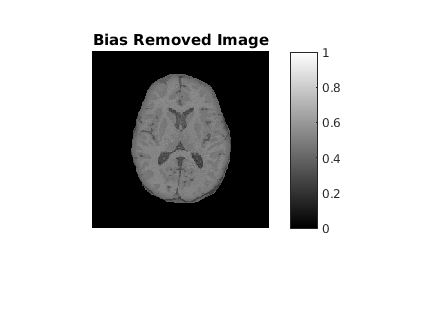
\includegraphics[]{biasRemoved}
\end{figure}

\begin{figure}[h]
\centering
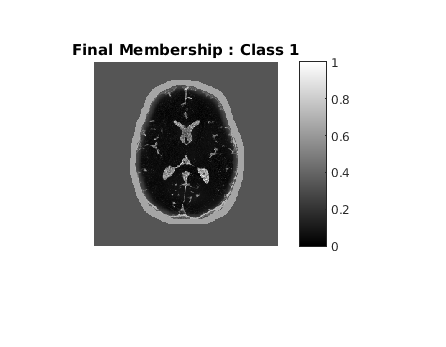
\includegraphics[]{fin1}
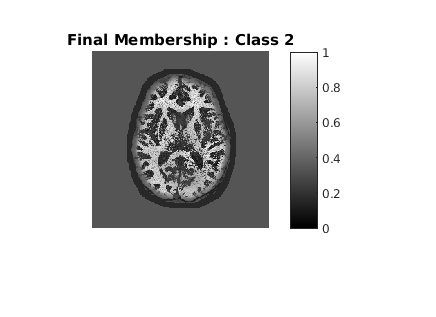
\includegraphics[]{fin2}
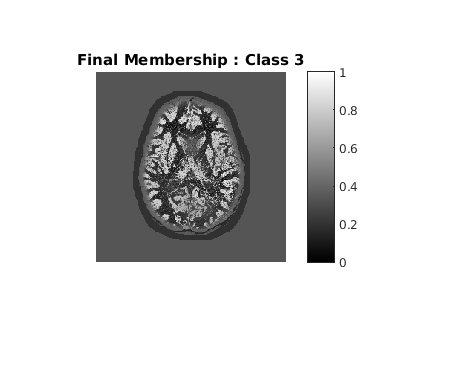
\includegraphics[]{fin3}
\end{figure}


\subsection{}
Final estimate of means = [0.1515  ,  0.4628  ,  0.5582]



\end{document}
